%%%%%%%%%%%%%%%%%%%%%%%%%%%%%%%%%%%%%%%%%%%%%%%%%%%%%%%%%%%%%%%%%%%%%%%%%%%%%%%%
% Template for USENIX papers.
%
% History:
%
% - TEMPLATE for Usenix papers, specifically to meet requirements of
%   USENIX '05. originally a template for producing IEEE-format
%   articles using LaTeX. written by Matthew Ward, CS Department,
%   Worcester Polytechnic Institute. adapted by David Beazley for his
%   excellent SWIG paper in Proceedings, Tcl 96. turned into a
%   smartass generic template by De Clarke, with thanks to both the
%   above pioneers. Use at your own risk. Complaints to /dev/null.
%   Make it two column with no page numbering, default is 10 point.
%
% - Munged by Fred Douglis <douglis@research.att.com> 10/97 to
%   separate the .sty file from the LaTeX source template, so that
%   people can more easily include the .sty file into an existing
%   document. Also changed to more closely follow the style guidelines
%   as represented by the Word sample file.
%
% - Note that since 2010, USENIX does not require endnotes. If you
%   want foot of page notes, don't include the endnotes package in the
%   usepackage command, below.
% - This version uses the latex2e styles, not the very ancient 2.09
%   stuff.
%
% - Updated July 2018: Text block size changed from 6.5" to 7"
%
% - Updated Dec 2018 for ATC'19:
%
%   * Revised text to pass HotCRP's auto-formatting check, with
%     hotcrp.settings.submission_form.body_font_size=10pt, and
%     hotcrp.settings.submission_form.line_height=12pt
%
%   * Switched from \endnote-s to \footnote-s to match Usenix's policy.
%
%   * \section* => \begin{abstract} ... \end{abstract}
%
%   * Make template self-contained in terms of bibtex entires, to allow
%     this file to be compiled. (And changing refs style to 'plain'.)
%
%   * Make template self-contained in terms of figures, to
%     allow this file to be compiled. 
%
%   * Added packages for hyperref, embedding fonts, and improving
%     appearance.
%   
%   * Removed outdated text.
%
%%%%%%%%%%%%%%%%%%%%%%%%%%%%%%%%%%%%%%%%%%%%%%%%%%%%%%%%%%%%%%%%%%%%%%%%%%%%%%%%

\documentclass[letterpaper,twocolumn,10pt]{article}
\usepackage[left=2cm, right=2cm, top=2cm, bottom=2cm]{geometry}
\usepackage{placeins}
\usepackage[shortlabels]{enumitem}
\usepackage{multirow}
\usepackage[table,xcdraw]{xcolor}
\usepackage{minted}
% color the table
\PassOptionsToPackage{table}{xcolor}
\usepackage{colortbl}
\usepackage{float}
% table number
\usepackage{caption}

% to be able to draw some self-contained figs
\usepackage{tikz}
\usepackage{amsmath}

% inlined bib file
\usepackage{filecontents}

%-------------------------------------------------------------------------------
\begin{document}
%-------------------------------------------------------------------------------

%don't want date printed
\date{}

% make title bold and 14 pt font (Latex default is non-bold, 16 pt)
\title{\Large \bf CS221 Project Performance Report of a System}

%for single author (just remove % characters)
\author{
{\rm Yucheng Wang}
\and
{\rm Ziyu Tang}
} % end author

\maketitle

%-------------------------------------------------------------------------------
\begin{abstract}
%-------------------------------------------------------------------------------

\end{abstract}


%-------------------------------------------------------------------------------
\section{Introduction}
%-------------------------------------------------------------------------------
\hspace{2em}For this project, we are evaluating a personal computer with an Ubuntu 20.04 system. We are mainly going to use bash script, C and C++ to implement our measurement on CPU cache size, I/O speed, bus speed, etc. The gcc version for C compiler is 9.3.0. The GNU bash is version 5.0.17(1)-release. To ensure the progress of this project, we are setting up subgoals for each week and zoom meetings (or in-person meetings) to discuss weekly objectives. As for the current week, we are mainly looking into useful commands to retrieve relevant hardware information and completing checkpoint 1. Additionally, we are planning on spending 2 hours per week. 

%-------------------------------------------------------------------------------
\section{Measurement Tool}
%-------------------------------------------------------------------------------
\hspace{2em}We are listing commands and measurement tools that are used to print out basic specifications of our system. As the project progresses, we will be using bash script, C and C++ to implement our own measurement for in-depth details of each hardware and software.
\begin{itemize}
  \vspace{-0.2cm}\item Check bash version:		bash --version
  \vspace{-0.2cm}\item Check gcc version:		gcc --version
  \vspace{-0.2cm}\item Check RAM speed:		sudo dmidecode --type 17
  \vspace{-0.2cm}\item PC specification:		hwinfo
  \vspace{-0.2cm}\item Device details:			sudo lshw -short
\end{itemize}


%-------------------------------------------------------------------------------
\section{Machine Description}
%-------------------------------------------------------------------------------
Using existing measuring tool from the system, we retrieve the following spec list for our machine. Notice since both disks are SSDs, there is no RPM for their specification.
% Please add the following required packages to your document preamble:
% \usepackage[table,xcdraw]{xcolor}
% If you use beamer only pass "xcolor=table" option, i.e. \documentclass[xcolor=table]{beamer}
\begin{table}[h!]
\centering
\begin{tabular}{ll}
\hline
\multicolumn{2}{c}{\cellcolor[HTML]{ABB2B9}CPU}                                                                                                  \\ \hline
\cellcolor[HTML]{D5D8DC}Mode               & AMD Ryzen 9 5900X                                                                                   \\
\cellcolor[HTML]{D5D8DC}Cycle Time         & \begin{tabular}[c]{@{}l@{}}a single FMA takes 4 cycles \\ with a throughput of 2/clock\end{tabular} \\
\cellcolor[HTML]{D5D8DC}L1d cache          & 384 KiB                                                                                             \\
\cellcolor[HTML]{D5D8DC}L1i cache          & 384 KiB                                                                                             \\
\cellcolor[HTML]{D5D8DC}L2 cache           & 6 MiB                                                                                               \\
\cellcolor[HTML]{D5D8DC}L3 cache           & 64 MiB                                                                                              \\
\cellcolor[HTML]{D5D8DC}I/O Bus            & PCIe 4.0                                                                                            \\
\cellcolor[HTML]{D5D8DC}Memory Bus         & 64 bits, 3600 mhz                                                                                   \\
\multicolumn{2}{c}{\cellcolor[HTML]{ABB2B9}Disk}                                                                                                 \\
\cellcolor[HTML]{D5D8DC}Model               & \begin{tabular}[c]{@{}l@{}}Disk1 Samsung SSD 970 EVO Plus\\ Disk2 Samsung SSD 860\end{tabular}      \\
\cellcolor[HTML]{D5D8DC}controller cache size  & $>$ 1 GB - 2 GB                                                                                  \\
\cellcolor[HTML]{D5D8DC}Capacity           & 4 TB (2 * 2 TB)                                                                                     \\ \hline
\multicolumn{2}{c}{\cellcolor[HTML]{ABB2B9}RAM}                                                                                                  \\
\cellcolor[HTML]{D5D8DC}Size               & 32 GB (2 * 16 GB)                                                                                   \\
\cellcolor[HTML]{D5D8DC}Total Width        & 64 bits                                                                                             \\
\cellcolor[HTML]{D5D8DC}Type               & DDR4                                                                                                \\
\cellcolor[HTML]{D5D8DC}Memory Technology  & DRAM                                                                                                \\
\cellcolor[HTML]{D5D8DC}Speed              & 2133 MT/s                                                                                           \\
\cellcolor[HTML]{D5D8DC}Form Factor        & DIMM                                                                                                \\
\multicolumn{2}{c}{\cellcolor[HTML]{ABB2B9}Network Card}                                                                                         \\
\cellcolor[HTML]{D5D8DC}Speed              & \begin{tabular}[c]{@{}l@{}}Wi-Fi6, a single\\ stream at 3.5 Gbps\end{tabular}                       \\
\multicolumn{2}{c}{\cellcolor[HTML]{ABB2B9}Operating System}                                                                                     \\
\cellcolor[HTML]{D5D8DC}Release \& Version & Ubuntu 20.04 (August 26, 2021)                                                                                       \\
                                           &                                
\end{tabular}
\caption{System Configuration}
\end{table}

%-------------------------------------------------------------------------------
\section{Experiments}


\subsection{CPU, Scheduling and OS Services}
For the following measurement operation, we are using existing command for the time being.
\begin{enumerate}
	\item Measurement overhead:\\
	For measuring overhead of reading time, we may use \mintinline{MySQL}{rdtscp} or \mintinline{MySQL}{rdtsc} to measure fine-grained operations this these.
	We may setup timestamp before reading and after reading to measure the difference in time.
	\item Procedure call overhead:\\
	For measuring procedure call, we may use \mintinline{MySQL}{rdtscp} or \mintinline{MySQL}{rdtsc} to measure fine-grained operations this these.
	We may setup timestamp before increment and after increment to measure the difference in time.
	\item System call overhead:\\
	For system call and kernel operation, we may use \mintinline{MySQL}{rdtscp} or \mintinline{MySQL}{rdtsc} to measure fine-grained operations this these.
	\item Task creation time:\\
	For task creation and execution time measurement, we can add \mintinline{MySQL}{time} before the command. For more specific program or method, we may set timestamp to measure time differences.
	
	\item Context switch time:\\
	We can setup a program that takes 2 processes, P1 and P2. Right after finishing executing P1, we switch to P2 to continue our execution. During these operation, we could set timestamp to measure time differences.
\end{enumerate}

\subsection{Memory}
\subsubsection{RAM access time}
\begin{enumerate}[\bfseries (a), wide, labelwidth=!, labelindent=0pt]
    \item \textbf{Methodology}\\
    To test out the access time for RAM, we allocate memory for different array sizes and assign different stride sizes to spread each element away. Depending on the allocation size, the allocation will happen in the l1 cache, l2 cache or main memory. Different stride sizes also provide different spatial locality. With smaller stride size, the spatial locality is higher; namely, the access time is quicker and vice versa. Below we define each function that in our algorithm:\\
    \hline \hline 
    \noindent\mintinline{C}{void access_time();}\\
    In this function, we use a nested for loop over two globally defined arrays and test out each combination of arr\_size and stride\_size by feeding into \mintinline[breaklines, breakafter=_]{C}{cache_access_time();}.

    \noindent\mintinline[breaklines, breakafter=_]{C}{void cache_access_time(int array_size, int stride);}\\
    In this function, we first allocate an array with the given size. Then, we initialize the array sequentially with elements being the gap of the stride size between each adjacent element. We take the mode over the number of elements to avoid possible segmentation faults. The actual measurement is carried out by accessing the array repeatedly and using the element as the next index. This way we are ensuring the measurement does not interfere with any other operations such as generating a random index to access or reading off another array. We repeat the operation 10000000 times and then take the average over every one million operations. This is done intentionally since the access is too short even in milliseconds. We argue this is still a fair measurement since to get the access over 1 operation, just divide the result by a million. Below it’s the current global array for testing.
    
    \noindent\mintinline[breaklines, breakafter=_]{C}{int arr_size[6] = {512 ,1024, 8192, 32768, 524288, 1048576};}\\
    \noindent\mintinline[breaklines, breakafter=_]{C}{int stride_size[5] = {4, 16, 64, 128, 1024};}\\
    \hline \hline 

    
    \item \textbf{Units}\\
    The measurement is done in million operation / milliseconds (ms).
    \item \textbf{Results}\\
    \textit{(*NOTICE: This is only a result showcased by doing preliminary tests. More detailed and extensive tests with larger test cases will be carried out for the final report.*)}
    \vspace{-0.5cm}
\begin{table}[h]
\begin{tabular}{|c|c|c|}
\hline
\textbf{Stride Size}   & \multicolumn{1}{l|}{\textbf{Array Size (kb)}} & \multicolumn{1}{l|}{\textbf{Latency (mil/ms)}} \\ \hline
                       & {\color[HTML]{434343} 512}                    & {\color[HTML]{434343} 1.512025}       \\ \cline{2-3} 
                       & 1024                                          & {\color[HTML]{434343} 1.449172}       \\ \cline{2-3} 
                       & 8192                                          & {\color[HTML]{434343} 1.447357}       \\ \cline{2-3} 
                       & 32768                                         & {\color[HTML]{434343} 1.554252}       \\ \cline{2-3} 
                       & 524288                                        & {\color[HTML]{434343} 1.566631}       \\ \cline{2-3} 
\multirow{-6}{*}{4}    & 1048576                                       & {\color[HTML]{434343} 1.502035}       \\ \hline
                       & {\color[HTML]{434343} 512}                    & {\color[HTML]{434343} 1.516243}       \\ \cline{2-3} 
                       & 1024                                          & {\color[HTML]{434343} 1.482777}       \\ \cline{2-3} 
                       & 8192                                          & {\color[HTML]{434343} 1.489482}       \\ \cline{2-3} 
                       & 32768                                         & {\color[HTML]{434343} 2.466684}       \\ \cline{2-3} 
                       & 524288                                        & {\color[HTML]{434343} 3.620132}       \\ \cline{2-3} 
\multirow{-6}{*}{16}   & 1048576                                       & {\color[HTML]{434343} 3.660654}       \\ \hline
                       & {\color[HTML]{434343} 512}                    & {\color[HTML]{434343} 1.499667}       \\ \cline{2-3} 
                       & 1024                                          & {\color[HTML]{434343} 1.524477}       \\ \cline{2-3} 
                       & 8192                                          & {\color[HTML]{434343} 1.505690}       \\ \cline{2-3} 
                       & 32768                                         & {\color[HTML]{434343} 4.436418}       \\ \cline{2-3} 
                       & 524288                                        & {\color[HTML]{434343} 7.248706}       \\ \cline{2-3} 
\multirow{-6}{*}{64}   & 1048576                                       & {\color[HTML]{434343} 7.272318}       \\ \hline
                       & {\color[HTML]{434343} 512}                    & {\color[HTML]{434343} 1.535247}       \\ \cline{2-3} 
                       & 1024                                          & {\color[HTML]{434343} 1.641065}       \\ \cline{2-3} 
                       & 8192                                          & {\color[HTML]{434343} 1.689175}       \\ \cline{2-3} 
                       & 32768                                         & {\color[HTML]{434343} 3.991784}       \\ \cline{2-3} 
                       & 524288                                        & {\color[HTML]{434343} 6.903875}       \\ \cline{2-3} 
\multirow{-6}{*}{128}  & 1048576                                       & {\color[HTML]{434343} 6.979855}       \\ \hline
                       & {\color[HTML]{434343} 512}                    & {\color[HTML]{434343} 3.036848}       \\ \cline{2-3} 
                       & 1024                                          & {\color[HTML]{434343} 3.041727}       \\ \cline{2-3} 
                       & 8192                                          & {\color[HTML]{434343} 3.784612}       \\ \cline{2-3} 
                       & 32768                                         & {\color[HTML]{434343} 3.777941}       \\ \cline{2-3} 
                       & 524288                                        & {\color[HTML]{434343} 19.634751}      \\ \cline{2-3} 
\multirow{-6}{*}{1024} & 1048576                                       & {\color[HTML]{434343} 20.833094}      \\ \hline
\end{tabular}
\end{table}
\newline
We further present our result in a graph where we set the $log_2(array size)$ as the x-axis and the measured latency as the y-axis. We denote ss as the stride size. Each plot will be fixed to a stride size where the only variable is the array size.
\begin{figure}[h]
    \centering
    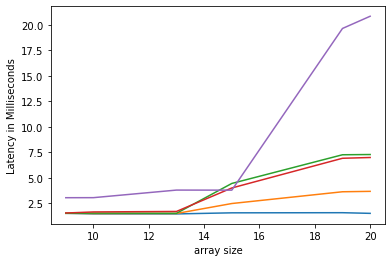
\includegraphics[width=70mm]{latency plot.png}
\end{figure}
    \item \textbf{Discussion}\\
    No base hardware performance at this time.\\
No prediction of the measured performance at this time.\\
We argue that the accuracy of our measurement is reliable since we ensure the measurement only contains accessing one array. All indices are retrieved from the array elements. We also take the average over a large amount of experiments, ruling out any outliers or instability in this measurement.\\
Observing the final result graph, at every stride size (plot), we can intuitively see two “jumps”: one at $log2(32768) = 15$ and the other at $log2(524288) = 19$. These two “jumps” are due to the fact that once the array reaches a certain size, the system will allocate it into either l1 cache, l2 cache or main memory.  Hence, this is the expected result as we increase the size of the array. 

\end{enumerate}
\newline
\subsubsection{RAM bandwidth}
\begin{enumerate}[\bfseries (a), wide, labelwidth=!, labelindent=0pt]
    \item \textbf{Methodology}\\
    For writing bandwidth, we want to measure the speed of assign elements into the array that is stored in the memory. Similarly, for reading bandwidth, we want to measure the speed of loading elements into the array that is stored in the memory. Below we define each function in our algorithm:\\
    \hline \hline 
    \noindent\mintinline{C}{void bandwidth();}\\
    In this function, we initialize an array in the memory with a length of 6000000 (maximum size without producing a segmentation fault). Then we carry out the measurement for writing bandwidth and reading bandwidth separately. For writing bandwidth, we sequentially assign an integer into the elements of the array. With a hand-unrolled loop, we store five integers at a time for each loop. A similar operation is done for reading bandwidth measurement as well except for this time we are reading the elements of the array sequentially instead of storing them. We record the time spent for these two for loop and then repeat these two operations 1000 times. To get the result, we take the average recorded time over 1000 times. Then we calculate the raw size of the array in bytes and divide it by the average recorded time. This way, we are calculating the read/write bandwidth in a unit of Bytes (bytes) / Milliseconds (ms).
    \hline \hline 
    \item \textbf{Units}\\
    The measurement is done in bytes (bytes) / milliseconds (ms).
    \item \textbf{Results}\\
    We present out result in a table below.
    \begin{table}[h]
    \begin{tabular}{|c|c|}
    \hline
    \textbf{Operation} & \textbf{Bandwidth (bytes/ms)} \\ \hline
    Writing            & 2588653.326821                \\ \hline
    Reading            & 2964002.620893                \\ \hline
    \end{tabular}
    \end{table}
    \item \textbf{Discussion}\\
    No base hardware performance at this time.\\
    No prediction of the measured performance at this time.\\
    We argue that the accuracy of our measurement is reliable since we carried out the simplest writing and reading operation to ensure there is little to none overhead being measured to destabilize our result. One such technique is by using loop unrolling, which accesses 5 elements at each iteration. This method reduces the number of instructions executed between executions of the loop branch logic. Overall, the number of iterations can be significantly reduced, making the measurement somewhere faster.\\
    An interesting fact in our output is that the reading bandwidth is larger than the writing bandwidth. This is indeed an expected difference since writing operations requires finding and allocating sufficient space and verifying the storage. This is much more expensive than simply reading off the memory.

\end{enumerate}
\newline
\subsubsection{Page fault service time}
\begin{enumerate}[\bfseries (a), wide, labelwidth=!, labelindent=0pt]
    \item \textbf{Methodology}\\
    Generally, page fault occurs when a process tries to access a block of memory that is not yet stored in the physical memory. The system must handle the page fault by locating the data in virtual memory and storing it from the physical memory. To recreate this handling process, we manually evoke such mistakes. Below we define each function in our algorithm:
    \hline \hline 
    \noindent\mintinline{C}{void page_fault();}\\
    Before running the function, we make sure the directory has a file with a size of 2 gigabytes called “largefile”. This is used to initialize a file descriptor that has to be mapped. In this function we use mmap() to map a file to a virtual address space. The number of bytes which need to be mapped is set to exactly the size of a page. The function mmap() returns the mapping in the virtual address space. The mapping then will be accessed 1000 times. We specifically define an offset that is two times larger than a page size. Hence, each time we try to access the mapping will result in a page fault. We record the time of the 1000 assessment and take the average of it which will produce a reliable result of page fault service time.
    \hline \hline 
    \item \textbf{Units}\\
    The measurement is done in milliseconds (ms).
    \item \textbf{Results}\\
    We present out result in a table below.
    \begin{table}[h]
\begin{tabular}{|l|l|}
\hline
\textbf{Operation} & \textbf{average time(ms)} \\ \hline
Page fault         & 0.000480                  \\ \hline
\end{tabular}
\end{table}
\newline
    \item \textbf{Discussion}\\
    No base hardware performance at this time.\\
No prediction of the measured performance at this time.\\
We argue that the accuracy of our measurement is reliable since we manually produce a page fault by using mmap() and accessing the memory outside mapping. The system will evoke the page fault handler. The service time will be recorded and averaged over 1000 times.\\
Comparing the latency of accessing a byte from main memory from the first part (RAM access time), you can intuitively see the result is significantly larger when a page fault needs to be handled. To be more specific, the latency of accessing one byte in the first part can be measured by dividing any result given by using the array size larger or equal to 524288kb by 10e6. For instance, when stride size is 128, with array size of 524288kb, accessing one byte should be 0.00000690387ms which is faster than accessing with page fault for almost 70 times.

\end{enumerate}

\newline
\subsection{Network}

\subsection{File System}

%%%%%%%%%%%%%%%%%%%%%%%%%%%%%%%%%%%%%%%%%%%%%%%%%%%%%%%%%%%%%%%%%%%%%%%%%%%%%%%%
\end{document}
%%%%%%%%%%%%%%%%%%%%%%%%%%%%%%%%%%%%%%%%%%%%%%%%%%%%%%%%%%%%%%%%%%%%%%%%%%%%%%%%

%%  LocalWords:  endnotes includegraphics fread ptr nobj noindent
%%  LocalWords:  pdflatex acks